\documentclass[../report.tex]{subfiles}

\begin{document}
\chapquote{Of chess, it has been said that life is not long enough for it, but that is the fault of life, not chess.}{William Napier}
\chapter{Recognising chess positions}
\label{chap:chess_recognition}
\begin{wrapfigure}[24]{r}{0pt}
    \centering
    \begin{tikzpicture}[
        node distance = 2cm,
        every text node part/.style={align=center},
        io/.style = {
            trapezium,
            trapezium left angle=70,
            trapezium right angle=110,
            minimum width=3cm,
            minimum height=1cm,
            text centered,
            draw=black
        },
        process/.style = {
            rectangle,
            minimum width=3cm,
            minimum height=1cm,
            text centered,
            draw=black
        },
        arrow/.style = {
            ->,>=stealth
        }
    ]
        \node[io] (input) {input image};
        \node[process,below=.5cm of input] (localisation) {chessboard localisation\\(\cref{sec:board_localisation})};
        \node[process,below of=localisation] (occupancy) {occupancy classification\\(\cref{sec:occupancy_classification})};
        \node[process,below of=occupancy] (piece) {piece classification\\(\cref{sec:piece_classification})};
        \node[process,below of=piece] (probabilities) {process probabilities\\(\cref{sec:preparing_results})};
        \node[io,below=.5cm of probabilities] (output) {\acs{fen} output};

        \draw[arrow] (input) -- (localisation);
        \draw[arrow] (localisation) -- node[right] {corner points} (occupancy);
        \draw[arrow] (occupancy) -- node[right] {occupancy mask} (piece);
        \draw[arrow] (piece) -- node[right] {piece probabilities} (probabilities);
        \draw[arrow] (probabilities) -- (output);
    \end{tikzpicture}
    \caption{Overview of the chess recognition pipeline.}
    \label{fig:chess_recognition_pipeline_overview}
\end{wrapfigure}
The chess recognition system is responsible for taking an \gls{rgb} image of a chessboard with pieces on it and  ultimately produce a \gls{fen} string representing the predicted chess position.
The pipeline, depicted in \cref{fig:chess_recognition_pipeline_overview}, consists of four main stages which shall be described in detail in the subsequent sections.

The first step is locating the chessboard in the image.
More specifically, we are interested in finding the pixel coordinates of the four chessboard corners. 
Using these corner points, we warp the image such that the chessboard forms a regular square grid, to eliminate perspective distortion in the sizes of the chess squares.
Next, we train a binary \gls{cnn} classifier to determine individual squares' occupancies.
Each of the occupied squares are then be input to another \gls{cnn} that is responsible for determining the type of piece. 
Finally, we use the output probabilities of the piece classifier to produce a \gls{fen} string representing the position. 


\section{Board localisation}
\label{sec:board_localisation}
To determine the location of the chessboard's corners, we shall rely on its regular geometric nature. 
Each square on the physical chessboard has the same width and height, even though their observed dimensions in the input image vary due to 3D perspective distortion.

\subsection{Finding intersection points}
\label{sec:find_intersection_points}
A chessboard consists of 64 squares that are arranged in an $8\times 8$ grid.
Thus, there are nine horizontal and nine vertical lines.
In the first step of our algorithm, we would like to detect the majority of these lines and find their intersection points.
Before conducting any futher computation, we resize the image to a width of 1,200 pixels, keeping the aspect ratio.

\subsubsection{Edge detection}
\begin{figure}
    \centering
    \begin{subfigure}[t]{0.47\textwidth}
        \centering
        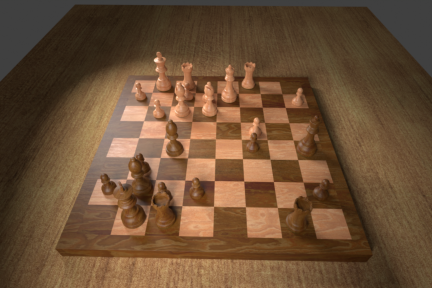
\includegraphics[width=\textwidth]{3828_corners_orig}
        \caption{original image}
    \end{subfigure}
    \hfill
    \begin{subfigure}[t]{0.47\textwidth}
        \centering
        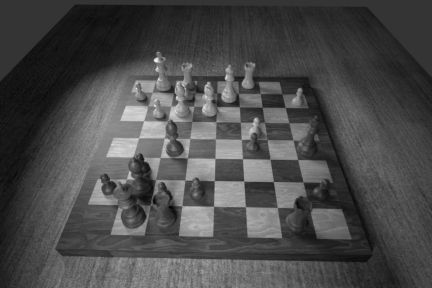
\includegraphics[width=\textwidth]{3828_corners_gray}
        \caption{grayscale image}
    \end{subfigure}
    \bigskip
    \begin{subfigure}[t]{0.47\textwidth}
        \centering
        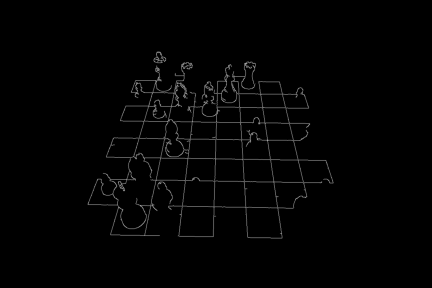
\includegraphics[width=\textwidth]{3828_corners_edges}
        \caption{detected edges}
        \label{fig:board_localisation_line_detection_edges}
    \end{subfigure}
    \hfill
    \begin{subfigure}[t]{0.47\textwidth}
        \centering
        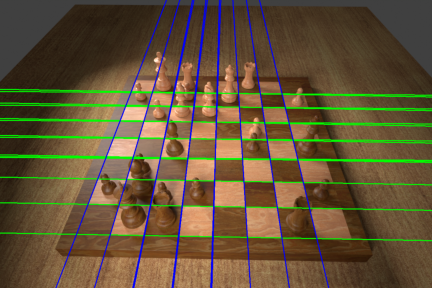
\includegraphics[width=\textwidth]{3828_corners_lines}
        \caption{detected lines, clustered into horizontal (green) and vertical (blue) lines}
        \label{fig:board_localisation_line_detection_horizontal_vertical}
    \end{subfigure}
    \bigskip
    \begin{subfigure}[t]{0.47\textwidth}
        \centering
        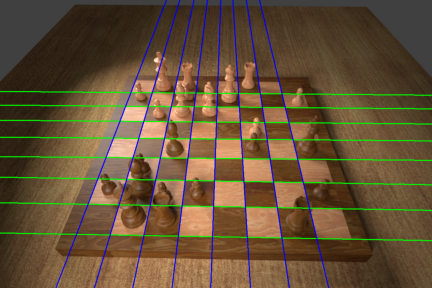
\includegraphics[width=\textwidth]{3828_corners_lines_clustered}
        \caption{elimination of similar lines}
        \label{fig:board_localisation_line_detection_elimination}
    \end{subfigure}
    \hfill
    \begin{subfigure}[t]{0.47\textwidth}
        \centering
        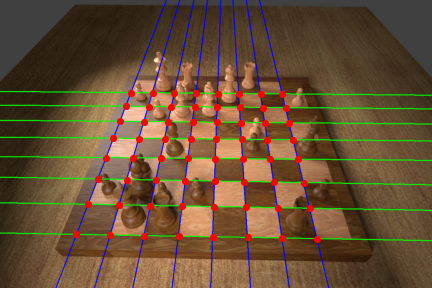
\includegraphics[width=\textwidth]{3828_corners_intersection_points}
        \caption{intersection points (red)}
        \label{fig:board_localisation_line_detection_intersections}
    \end{subfigure}
    \caption{The process of determining the intersection points on the chessboard.}
    \label{fig:board_localisation_line_detection}
\end{figure}
To detect edges in the input image, we convert the \gls{rgb} image to grayscale and apply the Canny edge detector \cite{canny1986}, the result of which is shown in \cref{fig:board_localisation_line_detection_edges}.
Canny edge detection is a multi-stage algorithm that first reduces noise in the image (by applying a Gaussian blur), then computes pixel intensity gradients, performs non-maximum supression, and finally refines the results using hysteresis thresholding \cite{canny1986}, although the precise details of this algorithm go beyond the scope of this report.

\subsubsection{Line detection}
\begin{figure}
    \centering
    \begin{tikzpicture}
        \begin{axis}[
            y dir = reverse,
            axis lines = center,
            xmin = 0, xmax = 4.5,
            ymin = 0, ymax = 2.5,
            xlabel = $x$,
            ylabel = $y$,
            xlabel style = {anchor=west},
            ylabel style = {anchor=north, at={(0,0)}},
            xtick = {0},
            ytick = {0},
            extra x ticks = 0,
            extra x tick style = {
                tick label style={
                    anchor=south east,
                    at={(-.1,-.1)}
            }},
            x=1cm,
            y=1cm,
            no markers
        ]
            \addplot {.5*-x + 2};
            \coordinate (O) at (0,0);
            \coordinate (A) at (.8,1.6);
            \coordinate (B) at (4,0);
            \draw[->] (O) -- (A) node[pos=.7,left] {$\rho$};
            \pic[draw, "$\theta$", <-, angle eccentricity=.6, angle radius=.7cm] {angle = A--O--B};
            \markRightAngle[size=8pt](B,A,O);
        \end{axis}
    \end{tikzpicture}
    \caption[A line in Hesse normal form.]{A line in Hesse normal form is parameterised by the angle $\theta$ to the $x$-axis and distance $\rho$ from the origin. The line is defined by the equation $\rho = x \cos \theta + y \sin \theta$. Equivalently, in slope-intercept form, we have $y = -x \cot \theta + \frac{\rho}{\sin \theta}$ provided that $\cos \theta \neq 0$, i.e.\ $\theta$ is not a multiple of $\pi$. Notice that the $y$-axis is pointing down because the origin of the coordinate system is the top left of the image.}
    \label{fig:hesse_normal_form}
\end{figure}
Next, we perform the Hough transform \cite{hough1962,duda1972} in order to detect lines that are formed by the edges.
To this end, we represent lines in Hesse normal form, meaning that they are parameterised by the angle $\theta$ that their normal vector forms with the $x$-axis, and the distance $\rho$ to the origin.
\Cref{fig:hesse_normal_form} explains this geometrically and gives rise to the equation of a line in Hesse normal form,
\begin{equation}
    \label{eq:hesse_normal_form}
    \rho = x \cos \theta + y \sin \theta.
\end{equation}
In fact, for a particular point $(x,y)$, \cref{eq:hesse_normal_form} represents the family of lines passing through it.
Here, each pair of $(\rho, \theta)$ values represents one particular line, and we only need to consider pairs where $\rho \geq 0$ and $0 \leq \theta < 2 \pi$ to parameterise all lines.

\begin{figure}
    \centering
    \begin{subfigure}[t]{0.4\textwidth}
        \begin{tikzpicture}
            \begin{axis}[
                y dir=reverse,
                xmin=0, 
                ymin=0, ymax=6,
                xlabel={$x$},
                ylabel={$y$},
                x=1cm,
                y=1cm
            ]
                \addplot+[mark=*] coordinates {(1,5)};
                \addplot+[mark=*] coordinates {(2,3)};
                \addplot+[mark=*] coordinates {(3,1)};
                \addplot[mark=none, dashed] {-2*x+7};
            \end{axis}
        \end{tikzpicture}
        \caption{three points in image space}
        \label{fig:hough_points_image_space}
    \end{subfigure}
    \hfill
    \begin{subfigure}[t]{0.56\textwidth}
        \begin{tikzpicture}
            \begin{axis}[
                no markers,
                xmin=0, xmax=6.28,
                ymin=0, ymax=6,
                samples=80,
                xlabel={$\theta$},
                ylabel={$\rho$},
                ylabel near ticks,
                yticklabel pos=right
            ]
                \addplot {1*cos(deg(x))+5*sin(deg(x))};
                \addplot {2*cos(deg(x))+3*sin(deg(x))};
                \addplot {3*cos(deg(x))+1*sin(deg(x))};
            \end{axis}
        \end{tikzpicture}
        \caption{lines passing through these three points in $(\rho,\theta)$ space}
        \label{fig:hough_points_parameter_space}
    \end{subfigure}
    \caption[An example of how lines in image space are represented in $(\rho,\theta)$ space.]{An example of how lines in image space are represented in $(\rho,\theta)$ space. The family of lines passing through a particular point in image space \subref{fig:hough_points_image_space} is represented by a sinusoid in $(\rho,\theta)$ space \subref{fig:hough_points_parameter_space}. The intersection point of the three curves represents the line passing through all three points.}
    \label{fig:hough_points}
\end{figure}
Plotting the pairs of $(\rho, \theta)$ values for a particular point in image space gives a sinusoidal curve that represents all lines passing through that point.
We can take multiple points in image space and plot their sinusoids. 
Then, each intersection in $(\rho, \theta)$ space represents a line passing through the corresponding points, as illustrated in \cref{fig:hough_points}.

For a given threshold $t$, the Hough transform essentially plots the sinusoids for all edge points in the input image (which we obtained using the Canny edge detection algorithm) and outputs intersection points in $(\rho,\theta)$ space that are on at least $t$ different sinusoids.
Consequently, the lines identified by the Hough transform are supported by at least $t$ edge points in the image.

\subsubsection{Filtering and clustering the lines}
On the chessboard images, the Hough transform typically yields around 200 lines, most of which are very similar. 
We first split them into horizontal and vertical lines and then eliminate similar lines.
Experiments showed that simply setting thresholds for the angle $\theta$ is insufficient for robustly classifying lines as horizontal or vertical.
This is because the camera is often tilted quite severely in the synthetic dataset as a result of the procedure outlined in \cref{sec:data_chess_positions} (and might be the case in real chessboard photos taken by humans, too).
Instead, we employ agglomerative clustering which is a bottom-up hierarchical clustering algorithm.
In this algorithm, each line starts off in its own cluster, and as the algorithm progresses, pairs of clusters are merged in a manner that aims to minimise the variance within the clusters.
We cluster the lines based only on their direction, i.e.\ their angle $\theta$, and use the smallest angle between two given lines as the distance metric.
Finally, we use the mean angle of both top-level clusters to determine which cluster represents the vertical lines and which the horizontal lines.
The clustered lines are depicted in \cref{fig:board_localisation_line_detection_horizontal_vertical}.

Next, we must eliminate similar lines by finding clusters of similar lines.
To eliminate similar horizontal lines, we first find the mean vertical line by considering the $\rho$ and $\theta$ values associated to the lines in the vertical cluster.
Then, we find the intersection points of all the horizontal lines with the mean vertical line and perform a DBSCAN clustering \cite{ester1996} to group similar lines based on these intersection points.
We use the mean $\rho$ and $\theta$ values of the lines in each group to represent the final set of discovered horizontal lines. 
The same procedure is applied vice-versa for the vertical lines, the result of which is shown in \cref{fig:board_localisation_line_detection_elimination}.

\subsubsection{Intersection points}
It remains to find the intersection points of the horizontal and vertical lines.
Given two lines parameterised by $(\rho_1,\theta_1)$ and $(\rho_2,\theta_2)$ respectively, we can find their point of intersection by observing that their equations in Hesse normal form (\cref{eq:hesse_normal_form}) constitute a system of two linear equations that can be solved for $x$ and $y$. 
We have
\begin{align*}
    \rho_1 &= x \cos \theta_1 + y \sin \theta_1 \\
    \rho_2 &= x \cos \theta_2 + y \sin \theta_2.
\end{align*}
Rearranging for $x$ and $y$, we obtain after some algebraic manipulation that
\begin{align}
    \label{eq:hesse_intersection_1}
    x &= \frac{\rho_2 \sin \theta_1 - \rho_1 \sin \theta_2}{\cos \theta_2 \sin \theta_1 - \cos \theta_1 \sin \theta_2}, \\
    \label{eq:hesse_intersection_2}
    y &= \frac{\rho_2 \cos \theta_1 - \rho_1 \cos \theta_2}{\sin \theta_2 \cos \theta_1 - \sin \theta_1 \cos \theta_2}.
\end{align}
Finally, using \cref{eq:hesse_intersection_1,eq:hesse_intersection_2} on each pair of horizontal and vertical lines, we can find the intersection points as depicted in \cref{fig:board_localisation_line_detection_intersections}.

\subsection{Finding the homography}
\label{sec:find_homography}
Once we have obtained the intersection points, the next step is to project them on to a regular grid. 
Using this projection, known as a \emph{homography}, we can warp the original image to eliminate the perspective distortion. 

\subsubsection{Computing the homography matrix}
\label{sec:homography_matrix}
The projection is described by a \emph{homography matrix} $\mH \in \R^{3 \times 3}$ \cite{szeliski2011} mapping any point
$\vp$
from the original image to
the corresponding point
$\vp'$
in the warped image using the relation
\begin{equation}
    \label{eq:homography_matrix_relation}
    \mH
    \vp
    = q \vp'
\end{equation}
up to a scalar factor $q \in \R$.
Here, we consider $\vp$ and $\vp'$ as 2D \emph{homogenous coordinate vectors}, which are three-component vectors that extend the Euclidean plane with points at infinity. 
More practically, a point $(x,y)$ in Euclidean space corresponds to the set of homogenous coordinates
$\begin{bmatrix}
    q x & q y & q
\end{bmatrix}^\top$ for any $q \in \R,q \neq 0$.
In practical terms, we can thus convert a homogenous coordinate to the corresponding Euclidean coordinate by taking its first two components and dividing by the third.

To compute a homography, we require four source points on the original image and four corresponding destination points in the warped image.
We can choose four instersection points that lie on two distinct horizontal and two distinct vertical lines (according to the lines found in \cref{fig:board_localisation_line_detection_elimination}) and therefore represent a rectangle on the chessboard.
Let the $3 \times 4$ matrix $\mP$ contain these points' homogenous coordinates as column vectors in clockwise order.
Let $\mP'$ be a matrix of the same size as $\mP$ containing this rectangle's coordinates in clockwise order.
In the warped space, the squares of the chessboard will be of unit length. 
Therefore, we can map the four points from the original image to a rectangle whose top left vertex coincides with the origin and whose side lengths are $s_x$ and $s_y$ (see \cref{fig:homography_illustration}).
\begin{figure}
    \centering
    \begin{subfigure}[t]{0.6\textwidth}
        \begin{tikzpicture}[remember picture]
            \begin{axis}[
                y dir = reverse,
                axis lines = center,
                xmin = 0, %xmax = 4.5,
                ymin = 0, %ymax = 2.5,
                xlabel = $x$,
                ylabel = $y$,
                xlabel style = {anchor=west},
                ylabel style = {anchor=north, at={(0,0)}},
                ticks=none,
                enlargelimits=upper,
                x=1.2cm,
                y=1.2cm,
                no markers
            ]
                \addplot graphics[xmin=0,ymin=0,xmax=5,ymax=3] {3828_corners_intersection_points_sample.png};
                \begin{scope}[xscale=5,yscale=3]
                    \coordinate (homography_from1) at (0.303987,0.327397);
                    \coordinate (homography_from2) at (0.791654,0.341584);
                    \coordinate (homography_from3) at (0.212619,0.841484);
                    \coordinate (homography_from4) at (0.780833,0.858014);
                \end{scope}
            \end{axis}
        \end{tikzpicture}
        \caption{region of the original image}
    \end{subfigure}
    \hfill
    \begin{subfigure}[t]{0.38\textwidth}
        \begin{tikzpicture}[remember picture]
            \begin{axis}[
                y dir = reverse,
                axis lines = center,
                xmin = 0, xmax = 2,
                ymin = 0, ymax = 1.5,
                xlabel = $x$,
                ylabel = $y$,
                xlabel style = {anchor=west},
                ylabel style = {anchor=north, at={(0,0)}},
                xtick = {0},
                ytick = {0},
                extra x ticks = 0,
                extra x tick style = {
                    tick label style={
                        anchor=south east,
                        at={(-.1,-.1)}
                }},
                x=2cm,
                y=2cm,
                no markers,
                clip=false
            ]
                \coordinate (homography_to1) at (0,0);
                \coordinate (homography_to2) at (1,0);
                \coordinate (homography_to3) at (0,1);
                \coordinate (homography_to4) at (1,1);
                \draw[dashed] (homography_to1) rectangle (homography_to4);
                \node[above] at (.5, 1) {$s_x$};
                \node[right] at (1, .5) {$s_y$}; 
                \node at (0,2) {};
            \end{axis}
        \end{tikzpicture}
        \caption{warped image}
    \end{subfigure}
    \begin{tikzpicture}[remember picture,overlay]
        \draw[->,red,thick] (homography_from1) -- (homography_to1);
        \draw[->,red,thick] (homography_from2) -- (homography_to2);
        \draw[->,red,thick] (homography_from3) -- (homography_to3);
        \draw[->,red,thick] (homography_from4) -- (homography_to4);
    \end{tikzpicture}
    \caption{Projection of four intersection points from the original to the warped image.}
    \label{fig:homography_illustration}
\end{figure}
We have
\begin{equation*}
    \mP' = \begin{bmatrix}
        0 & 0 & 1 \\
        s_x & 0 & 1 \\
        s_x & s_y & 1 \\
        0 & s_y & 1
    \end{bmatrix}^\top.
\end{equation*}
Since the homography matrix maps points from the original image to the output image, we obtain from \cref{eq:homography_matrix_relation} the relation 
\begin{equation}
    \label{eq:homography_matrix_relation_corners}
    \mH \mP = \mP' (\mI_4 \vq)
\end{equation}
where the vector $\vq \in \R^4$ represents the scale factor for each point.
\Cref{eq:homography_matrix_relation_corners} describes a system of linear equations that we can solve computationally for $\mH$.
Then, we can use \cref{eq:homography_matrix_relation} to project all other intersection points to the warped image.

\subsubsection{Finding the optimal homography}
\label{sec:find_optimal_homography}
Although \cref{fig:board_localisation_line_detection_intersections} has no intersection points that are outliers (because all of the identified lines do, in fact, correspond to squares on the chessboard), our algorithm must be robust when facing lines identified in the image that do not correspond to squares on the chessboard.
\Cref{fig:incorrect_intersection_points} depicts one such example; however, in non-synthetic chessboard images, especially with other objects in the image that exhibit straight lines, there is often an even greater number of outliers. 
\begin{figure}
    \centering
    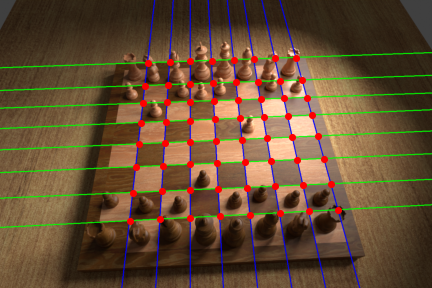
\includegraphics[width=\textwidth]{0064_corners_intersection_points.png}    
    \caption[A sample from the training set with an incorrectly identified line.]{A sample from the training set with an incorrectly identified line. The top horizontal line is at the border of the chessboard instead of the top chessboard squares.}
    \label{fig:incorrect_intersection_points}
\end{figure}

\Gls{ransac} \cite{fischler1981} is a non-deterministic iterative model fitting algorithm that can robustly estimate a model's parameters in such a manner that is not significantly influenced by outliers.
It can be applied to a variety of situations where a model must be fit to a dataset containing outliers.
In our case, the dataset consists of the intersection points (some of which are outliers due to detecting irrelevant lines) and the model is a homography that corresponds to the inlier intersection points.
The \gls{ransac} algorithm consists of two main steps:
\begin{enumerate}
    \item \label{enum:ransac_1}
        Randomly sample a set of observations from the dataset that contains the minimum number of samples sufficient to fit the model. 
        We require four points to compute a homography, so this is the number of intersection points we must sample in this step.
    \item \label{enum:ransac_2}
        Fit the model to these samples, and then determine which observations are explained by the model within some threshold (the threshold should be just large enough to account for the expected noise in the dataset). 
        This is the set of inliers, and if the size of this set is greater than the inliers discovered in the previous iteration, we will retain this model instead of the previous.
        Repeat from step 1 until reaching a specified number of iterations.
\end{enumerate}

Applied to our problem, choosing any four intersection points in step \ref{enum:ransac_1} would be quite unwise because we would not know which points they represent on the chessboard, making it infeasible to map them to the warped image such that the chess squares are snapped to the grid of whole numbers.
Instead, we randomly choose four points that we believe to form a rectangle on the chessboard.
This means that we select two horizontal and two vertical lines at random, and choose the four intersection points of these lines as the random sample.
We know that these four points form a rectangle in the warped image, so we can map to a rectangle as explained in \cref{sec:homography_matrix} and illustrated in \cref{fig:homography_illustration}.

\begin{algorithm}
    \begin{algorithmic}[1]
        \Input the set of intersection points $\sP \subset \R^2$
        \Parameters minimum number of iterations $i_\text{min}$, maximum number of iterations $i_\text{max}$, minimum number of inliers $c$, inlier threshold $\epsilon_\text{max}$
        \Output a bijective mapping $m : \sI \to \sW$ from a set of inlier points $\sI \subseteq \sP$ to a set of warped points $\sW \subset \mathbb{Z}^2$ that is given by its graph $\sM \subset \sI \times \sW$
        \State $\sP \gets \{h(\vp) : \vp \in \sP\}$ \Comment{convert to homogenous coordinates}
        \State $\sI, \sW, \sM \gets \emptyset, \emptyset, \emptyset$ \Comment{initialise outputs}
        \State $i \gets 0$ \Comment{number of iterations}
        \While{$(i < i_\text{min}) \vee (\abs{\sI} < c)$}
            \State $x_1,x_2 \gets \text{choose}(\{1, 2, \dots, x_\text{max}\})$ \Comment{randomly choose such that $x_1<x_2$}
            \State $y_1,y_2 \gets \text{choose}(\{1, 2, \dots, y_\text{max}\})$ \Comment{randomly choose such that $y_1<y_2$}
            \State $\vp_1,\vp_2,\vp_3,\vp_4 \gets$ intersection points in $\sP$ corresponding to the four points described by vertical lines $x_1,x_2$ and horizontal lines $y_1,y_2$ (in clockwise order)
            \State $\mP \gets \begin{bmatrix}
                \vp_1 & \vp_2 & \vp_3 & \vp_4
            \end{bmatrix}^\top$ \Comment{matrix of original points}
            \ForAll{$s_x \in \{1, 2, \dots, 8\}$}
                \label{alg:ransac:for_sx}
                \ForAll{$s_y \in \{1, 2, \dots, 8\}$}
                    \label{alg:ransac:for_sy}
                    \State $\mP' \gets \begin{bmatrix}
                        0 & 0 & 1 \\
                        s_x & 0 & 1 \\
                        s_x & s_y & 1 \\
                        0 & s_y & 1
                    \end{bmatrix}^\top$ \Comment{matrix of warped points}
                    \State $\mH \gets$ homography matrix calculated for $\mP$ and $\mP'$ using \cref{eq:homography_matrix_relation_corners}
                        \label{alg:ransac:compute_homography}
                    \State $\sI_C \gets \emptyset$ \Comment{candidate set of inliers for this iteration}
                    \State $\sW_C \gets \emptyset$ \Comment{candidate set of warped points}
                    \State $\sM_C \gets \emptyset$ \Comment{candidate mapping}
                    \ForAll{$\vp \in \sP$}
                        \label{alg:ransac:for_loop_over_all_points}
                        \Comment{iterate over all intersection points}
                        \State $\vp' \gets h^{-1}(\mH \vp)$ \Comment{warp the point according to our model}
                        \label{alg:ransac:warp}
                        \State $\vq \gets \text{round}(\vp')$ \Comment{snap to grid (round element-wise to nearest whole number)}
                        \If{$\vq \in \sW_C$} \Comment{ignore this point if we already mapped it}
                            \State \textbf{continue}
                        \EndIf
                        \State $\epsilon \gets \norm{\vp' - \vq}_1$ \Comment{calculate the error}\label{alg:ransac:error}
                        \If{$\epsilon \leq \epsilon_\text{max}$} \Comment{determine whether we have an inlier}
                            \State $\vp \gets h^{-1}(\vp)$
                            \State $\sI_C \gets \sI_C \cup \{\vp\}$ \Comment{add the inlier to our candidate mapping}
                            \State $\sW_C \gets \sW_C \cup \{\vq\}$
                            \State $\sM_C \gets \sM_C \cup \{(\vp, \vq)\}$
                        \EndIf
                    \EndFor
                    \If{$\abs{\sI_C} > \abs{\sI}$} \Comment{update the set of inliers if we found more}
                        \State $\sI,\sW,\sM \gets \sI_C,\sW_C,\sM_C$
                    \EndIf
                \EndFor
            \EndFor
            \IIf {$i\geq i_\text{max}$}
                \textbf{break}
            \EndIIf \Comment{guard against iterating indefinitely}
            \State $i \gets i + 1$
        \EndWhile
    \end{algorithmic}
    \caption{\acs{ransac}-based algorithm for finding the optimal homography.}
    \label{alg:ransac}
\end{algorithm}
The \gls{ransac}-based method of finding the inlier intersection points is described in \Cref{alg:ransac}. 
To simplify notation in the algorithm, we use the function $h : \R^2 \to \R^3$ to convert Euclidean coordinates to homogenous coordinates and $h^{-1} : \R^3 \to \R^2$ to denote the reverse operation.
Based on our characterisation of homogenous coordinates from \cref{sec:homography_matrix}, these functions can be defined as
\begin{equation*}
    h(x,y) = \begin{bmatrix}
        x\\y\\1
    \end{bmatrix}
\end{equation*}
and
\begin{equation*}
    h^{-1}(x,y,z) = \begin{bmatrix}
        \sfrac{x}{z}\\
        \sfrac{y}{z}
    \end{bmatrix}
\end{equation*}
provided that $z \neq 0$.

The input to \cref{alg:ransac} is the set of intersection points $\sP \subset \R^2$ in the original image.
Its output is a bijection $m : \sI \to \sW$ from a set of inlier points $\sI \subseteq \sP$ to a set of warped points $\sW \subset \mathbb{Z}^2$. 
Notice that the warped points are represented by two-dimensional vectors whose components are whole numbers, meaning that they lie on a grid of whole numbers.
Each square on the chessboard is represented by a square of unit length on the grid.
The chessboard itself is represented by a $8 \times 8$ square on that grid.
However, since the set of inliers likely does not contain all vertices of the chessboard squares (for example because some lines were not recognised as seen in \cref{fig:board_localisation_line_detection_elimination,fig:incorrect_intersection_points}) we do not yet know the location of that $8 \times 8$ square.

Once we have computed the output of \cref{alg:ransac} and obtained the mapping $m$ of points from the original image to points on the grid of the warped image, we can recompute the homography matrix $\mH$ using \cref{eq:homography_matrix_relation_corners} with \emph{all} inliers to obtain a more accurate homography that is based on more than just four points.
To do so, we take the matrix of original points $\mP$ to be a $3 \times \abs{\sI}$ matrix whose columns are populated with all the intersection points $\sI$ as homogenous coordinate vectors.
The matrix of warped points $\mP'$ of the same size is populated by the corresponding points in warped space $\sW$ according to the bijection $m$.
Using the new $\mP$ and $\mP'$ matrices, \cref{eq:homography_matrix_relation_corners} becomes an overdetermined linear system, so we compute $\mH$ as the least squared error solution instead of the exact solution.
Finally, we can use the homography matrix to project the pixels of the original image to obtain a warped image as in \cref{fig:homography_warped}. 
\begin{figure}
    \centering
    \begin{subfigure}[t]{0.55\textwidth}
        \begin{tikzpicture}
            \begin{axis}[
                y dir = reverse,
                axis lines = center,
                xmin = 0, %xmax = 4.5,
                ymin = 0, %ymax = 2.5,
                xlabel = $x$,
                ylabel = $y$,
                xlabel style = {anchor=west},
                ylabel style = {anchor=north, at={(0,0)}},
                ticks=none,
                enlargelimits=upper,
                x=2cm,
                y=2cm,
                no markers
            ]
                \addplot graphics[xmin=0,ymin=0,xmax=3,ymax=2] {3828_corners_intersection_points.png};
            \end{axis}
        \end{tikzpicture}
        \caption{original image with intersection points}
    \end{subfigure}
    \hfill
    \begin{subfigure}[t]{0.40\textwidth}
        \begin{tikzpicture}[remember picture]
            \begin{axis}[
                y dir = reverse,
                axis lines = center,
                xmin = 0, %xmax = 4.5,
                ymin = 0, %ymax = 2.5,
                xlabel = $x$,
                ylabel = $y$,
                xlabel style = {anchor=west},
                ylabel style = {anchor=north, at={(0,0)}},
                ticks=none,
                enlargelimits=upper,
                x=2cm,
                y=2cm,
                no markers
            ]
            \addplot graphics[xmin=0,ymin=0,xmax=2,ymax=2] {3828_corners_warped.png};
            \end{axis}
        \end{tikzpicture}
        \caption{warped image}
        \label{fig:homography_warped_warped}
    \end{subfigure}
    \caption[The original image is warped using the computed homography matrix $\mH$.]{The original image is warped using the computed homography matrix $\mH$. Detected lines and intersection points are overlaid in the original image as per \cref{fig:board_localisation_line_detection_elimination}. The corresponding intersection points are marked in red in the warped image and lie on a regular unit-length grid.}
    \label{fig:homography_warped}
\end{figure}

\subsubsection{Optimisations}
\Cref{alg:ransac} aims to outline the method of determining the inlier points in a manner that is easy to follow.
In practise, the employed algorithm is different in order to achieve improved performance.
Implementing these differences in \cref{alg:ransac} would have made it too convoluted to follow, so they shall instead briefly be summarised below:
\begin{itemize}
    \item The for loop on line \ref{alg:ransac:for_loop_over_all_points} can be vectorised and replaced by matrix operations.
    \item The computation of the homography matrix on line \ref{alg:ransac:compute_homography} occurs 64 times per iteration of the outer loop, due to the two for loops on lines \ref{alg:ransac:for_sx} and \ref{alg:ransac:for_sy}.
        Instead, it should be moved before the two aforementioned for loops and computed for the scale $s_x=s_y=1$.
        To ensure the points are mapped correctly, we must add the instruction $\vp' \gets \vp' \odot \begin{bmatrix}
            s_x & s_y
        \end{bmatrix}^\top$ immediately after line \ref{alg:ransac:warp} in order to scale the warped points.
    \item The for loops on lines \ref{alg:ransac:for_sx} and \ref{alg:ransac:for_sy} do not need to be nested; instead, one could first consider only the $x$-component of the vectors when calculating the errors for each scale $s_x$, and then do the same for the $y$-components and $s_y$.
        Finally, we would choose the best $s_x$ and $s_y$ (with the least accumulated error), compute the total error, and use the information to update the mappings if necessary.
        This is the reason for using the $\ell_1$ norm for computing the error on line \ref{alg:ransac:error}, since it can be easily decomposed into the two directional components.
\end{itemize}


\subsection{Inferring missing lines}
\label{sec:infer_missing_lines}
It was noted at the end of \cref{sec:find_optimal_homography} that while the result of \cref{alg:ransac} projects the inlier intersection points onto a regular grid of whole numbers, it does not explicitly indicate the location of the $8\times 8$ sub-grid that represents the chessboard.
To understand the set of inliers, we shall first compute the minimum and maximum $x$ and $y$ values of the warped points.
We shall use the notation
\begin{align}
    &x_\text{min} = \min \sW_x,
    &x_\text{max} = \max \sW_x,\label{eq:infer_lines_x_extrema}\\
    &y_\text{min} = \min \sW_y,
    &y_\text{max} = \max \sW_y,
\end{align}
where
\begin{equation}
    \sW_x = \left\{ x : \begin{bmatrix}
        x & y
    \end{bmatrix}^\top \in \sW \right\}%
    \qquad \text{and} \qquad%
    \sW_y = \left\{ y : \begin{bmatrix}
        x & y
    \end{bmatrix}^\top \in \sW \right\}.
\end{equation}
The $x_\text{min}$ value describes the leftmost vertical line in the warped image given by the equation $x=x_\text{min}$, and the value of $x_\text{max}$ describes the rightmost vertical line. 
Similarly, the values of $y_\text{min}$ and $y_\text{max}$ represent the top and bottom lines.
Examining the range of $x$-values ($x_\text{max}-x_\text{min}$) gives an indication of whether the vertical lines we identified represent the whole chessboard, part of it, or even a range that is wider than the chessboard itself, horizontally.
We thus distinguish between three cases based on the $x$-values which we shall outline below. 
\begin{caselist}
    \begin{case}{$x_\text{max}-x_\text{min}=8$}\label{case:infer_borders_equal}%
        In this case, no action is required because we detected the two outer vertical lines.
        The leftmost vertical line of the chessboard is located at $x=x_\text{min}$ and the rightmost line is at $x=x_\text{max}$ on the warped image.
    \end{case}

    \begin{case}{$x_\text{max}-x_\text{min}>8$}
        This case arises when the vertical line $x=x_\text{min}$ is to the left of the left edge of the chessboard and/or the vertical line $x=x_\text{max}$ is right of the right edge of the chessboard.
        In other words, the range of $x$-values covers more than just the chessboard.
        To remedy this, we iteratively update $\sW_x$ by applying
        \begin{equation*}
            \sW_x \gets \sW_x \setminus \{x_\text{min},x_\text{max}\}
        \end{equation*}
        and recomputing $x_\text{min}$ and $x_\text{max}$ by \cref{eq:infer_lines_x_extrema}
        until $x_\text{max}-x_\text{min}\leq 8$.
        Then, we update the set of warped points $\sW$ as
        \begin{equation*}
            \sW = \left\{
                \begin{bmatrix}
                    x & y
                \end{bmatrix}^\top
                :
                \begin{bmatrix}
                    x & y
                \end{bmatrix}^\top
                \in \sW, \ x \in \sW_x
            \right\},
        \end{equation*}
        retaining only the warped points whose $x$-component is in the interval $[x_\text{min},x_\text{max}]$.
        We also remove the corresponding points from $\sI$ and the mapping $m$'s graph $\sM$.
        Then, we fall either in case \ref{case:infer_borders_equal} or \ref{case:infer_borders_greater}, depending on the values of $x_\text{min}$ and $x_\text{max}$.
    \end{case}

    \begin{case}{$x_\text{max}-x_\text{min}<8$}\label{case:infer_borders_greater}%
        This most common scenario arises when the grid that should represent the chessboard in the warped image is smaller than eight units in width.
        \Cref{fig:homography_warped} illustrates this case and makes clear that it arises because either one or both of the outermost vertical lines were not detected on the chessboard. 
        Determining whether the grid should be expanded towards the left or the right involves futher processing of the image which shall be outlined below.
        
        We calculate the horizontal intensity gradients in the warped image for each pixel in order to determine whether an additional vertical line is more likely to occur one unit to the left or one unit to the right of the currently identified grid.
        To do so, we first convert the \gls{rgb} image to grayscale and then apply the horizontal Sobel filter which is a discrete differentiation operator that provides an approximation for the gradient intensity in the horizontal direction.
        Large horizontal gradient intensities give rise to vertical lines in the warped image which can be used in order to determine whether the chessboard should be expanded to the left or right.

        The Sobel filter is widely used in image processing and consists of two kernels that are convolved over the input image, a horizontal and a vertical one.
        Typically, the results of both convolution operations is calculated, and then some elementary trigonometry can be applied in order to determine the gradient directions for each pixel.
        However, since we are only interested in determining the gradients in the horizontal direction, it suffices to use the horizontal Sobel kernel
        \begin{equation}
            \mS_x = \begin{bmatrix}
                \label{eq:sobel_kernel_horizontal}
                +1 & 0 & -1\\
                +2 & 0 & -2\\
                +1 & 0 & -1
            \end{bmatrix}
        \end{equation}
        Given an intensity image (i.e.\ a grayscale image) of dimensions $h \times w$ that is represented by the matrix $\mA \in \R^{h\times w}$, 
        we compute the horizontal gradient intensity at each pixel by
        \begin{equation}
            \label{eq:sobel_operation_horizontal}
            \mG_x = \mS_x * \mA
        \end{equation}
        where $\mG_x$ is of the same dimensionality as $\mA$ and contains the computed gradient intensities.
        Then, we can apply the Canny edge detector (as we did in \cref{sec:find_intersection_points}) to image represented by $\mG_x$ in order to eliminate noise and obtain clear edges. 
        \begin{figure}
            \centering
            \begin{subfigure}[t]{0.48\textwidth}
                \begin{tikzpicture}
                    \begin{axis}[
                        y dir = reverse,
                        axis lines = center,
                        xmin = 0, %xmax = 4.5,
                        ymin = 0, %ymax = 2.5,
                        xlabel = $x$,
                        ylabel = $y$,
                        xlabel style = {anchor=west},
                        ylabel style = {anchor=north, at={(0,0)}},
                        ticks=none,
                        enlargelimits=upper,
                        x=5cm,
                        y=5cm,
                        no markers
                    ]
                        \addplot graphics[xmin=0,ymin=0,xmax=1,ymax=1] {3828_corners_warped.png};
                    \end{axis}
                \end{tikzpicture}
                \caption{warped image from \cref{fig:homography_warped_warped}}
            \end{subfigure}
            \hfill
            \begin{subfigure}[t]{0.48\textwidth}
                \begin{tikzpicture}[remember picture]
                    \begin{axis}[
                        y dir = reverse,
                        axis lines = center,
                        xmin = 0, %xmax = 4.5,
                        ymin = 0, %ymax = 2.5,
                        xlabel = $x$,
                        ylabel = $y$,
                        xlabel style = {anchor=west},
                        ylabel style = {anchor=north, at={(0,0)}},
                        ticks=none,
                        enlargelimits=upper,
                        x=5cm,
                        y=5cm,
                        no markers
                    ]
                    \addplot graphics[xmin=0,ymin=0,xmax=1,ymax=1] {3828_corners_warped_gray.png};
                    \end{axis}
                \end{tikzpicture}
                \caption{conversion to grayscale}
            \end{subfigure}

            \bigskip
            \begin{subfigure}[t]{0.48\textwidth}
                \begin{tikzpicture}
                    \begin{axis}[
                        y dir = reverse,
                        axis lines = center,
                        xmin = 0, %xmax = 4.5,
                        ymin = 0, %ymax = 2.5,
                        xlabel = $x$,
                        ylabel = $y$,
                        xlabel style = {anchor=west},
                        ylabel style = {anchor=north, at={(0,0)}},
                        ticks=none,
                        enlargelimits=upper,
                        x=5cm,
                        y=5cm,
                        no markers
                    ]
                        \addplot graphics[xmin=0,ymin=0,xmax=1,ymax=1] {3828_corners_warped_gradients_horizontal.png};
                    \end{axis}
                \end{tikzpicture}
                \caption{horizontal gradient intensities as computed by the Sobel operator (the colour scale shows low values in black and high values in white)}
            \end{subfigure}
            \hfill
            \begin{subfigure}[t]{0.48\textwidth}
                \begin{tikzpicture}[remember picture]
                    \begin{axis}[
                        y dir = reverse,
                        axis lines = center,
                        xmin = 0, %xmax = 4.5,
                        ymin = 0, %ymax = 2.5,
                        xlabel = $x$,
                        ylabel = $y$,
                        xlabel style = {anchor=west},
                        ylabel style = {anchor=north, at={(0,0)}},
                        ticks=none,
                        enlargelimits=upper,
                        x=5cm,
                        y=5cm,
                        no markers
                    ]
                    \addplot graphics[xmin=0,ymin=0,xmax=1,ymax=1] {3828_corners_warped_gradients_horizontal_edges.png};
                    \end{axis}
                \end{tikzpicture}
                \caption{result of Canny edge detection on the horizontal gradient image}
            \end{subfigure}
            \caption[Horizontal gradient intensities calculated on the warped image in order to detect vertical lines.]{Horizontal gradient intensities calculated on the warped image in order to detect vertical lines. The red dots overlaid on each image correspond to the intersection points in $\sI$. Here, $x_\text{max}-x_\text{min}=7$ because there are eight columns of points instead of nine. This is because the rightmost vertical line was not detected. Note that the algorithm also failed to detect the topmost horizontal line, but the horizontal lines are handled later (using vertical gradients).}
            \label{fig:warped_image_gradients}
        \end{figure}
        \Cref{fig:warped_image_gradients} shows the results of these operations on the running example.

        On that image we shall sum the pixel intensities on the vertical lines at $x=x_\text{min}-1$ and $x=x_\text{max}+1$ (with a small tolerance to the left and to the right).
        Then, if the sum of pixel intensities was greater at $x=x_\text{min}-1$ than $x=x_\text{max}+1$, we update $x_\text{min} \gets x_\text{min}-1$, or otherwise $x_\text{max} \gets x_\text{max}+1$.
        We repeat this process until $x_\text{max}-x_\text{min}=8$.
    \end{case}
\end{caselist}

Although the three cases above examine only the $x$-values to locate the horizontal position of the chessboard, it is trivial to see how this method applies to determine the vertical position of the chessboard using the $y$-values, too.
However, the main caveat the reader should acknowledge is that we must use the vertical sobel kernel
\begin{equation}
    \mS_x = \begin{bmatrix}
        +1 & +2 & +1\\
        0 & 0 & 0\\
        -1 & -2 & -1\\
    \end{bmatrix}.
\end{equation}
instead of the horizontal one given in \cref{eq:sobel_kernel_horizontal}, and as a consequence \cref{eq:sobel_operation_horizontal} becomes
\begin{equation}
    \mG_y = \mS_y * \mA.
\end{equation}

By following the instructions according to the three cases above for both the horizontal and vertical directions, we obtain the
$x_\text{min}$,
$x_\text{max}$,
$y_\text{min}$, and
$y_\text{max}$
values that describe the location of the chessboard in the warped image. 
As such, the coordinates of the four corners of the chessboard on the warped image can be expressed as
\begin{equation*}
    \begin{split}
        \vp'_1 &= \begin{bmatrix}
            x_\text{min} & y_\text{min}
        \end{bmatrix}^\top \\
        \vp'_3 &= \begin{bmatrix}
            x_\text{max} & y_\text{max}
        \end{bmatrix}^\top
    \end{split}
    \qquad\qquad
    \begin{split}
        \vp'_2 &= \begin{bmatrix}
            x_\text{max} & y_\text{min}
        \end{bmatrix}^\top \\
        \vp'_4 &= \begin{bmatrix}
            x_\text{min} & y_\text{max}
        \end{bmatrix}^\top.
    \end{split}
\end{equation*}
The points are supplied in clockwise order, starting from the top left.

Finally, we can use the inverse of the homography matrix in order to project these points back onto the original image by inverting \cref{eq:homography_matrix_relation}.
Notice that the points must be converted to homogenous coordinates and back again, so the equation becomes 
\begin{equation}
    \vp_i =
    h^{-1}\left(
        \mH^{-1}
        h(\vp'_i)
    \right)
\end{equation}
for $i=1,2,3,4$.
\begin{figure}
    \centering
    \begin{subfigure}[t]{0.48\textwidth}
        \begin{tikzpicture}
            \begin{axis}[
                y dir = reverse,
                axis lines = center,
                xmin = 0, %xmax = 4.5,
                ymin = 0, %ymax = 2.5,
                xlabel = $x$,
                ylabel = $y$,
                xlabel style = {anchor=west},
                ylabel style = {anchor=north, at={(0,0)}},
                ticks=none,
                enlargelimits=upper,
                x=5cm,
                y=5cm,
                no markers
            ]
                \addplot graphics[xmin=0,ymin=0,xmax=1,ymax=1] {3828_corners_warped_result.png};
            \end{axis}
        \end{tikzpicture}
        \caption{warped image with detected corner points $\vp'_i$}
    \end{subfigure}
    \hfill
    \begin{subfigure}[t]{0.48\textwidth}
        \begin{tikzpicture}[remember picture]
            \begin{axis}[
                y dir = reverse,
                axis lines = center,
                xmin = 0, %xmax = 4.5,
                ymin = 0, %ymax = 2.5,
                xlabel = $x$,
                ylabel = $y$,
                xlabel style = {anchor=west},
                ylabel style = {anchor=north, at={(0,0)}},
                ticks=none,
                enlargelimits=upper,
                x=1.67cm,
                y=1.67cm,
                no markers
            ]
            \addplot graphics[xmin=0,ymin=0,xmax=3,ymax=2] {3828_corners_unwarped_result.png};
            \end{axis}
        \end{tikzpicture}
        \caption{original image with reprojected corner points $\vp_i$}
    \end{subfigure}
    \caption{The identified corner points are projected back from the warped image onto the original image using the inverse homography matrix.}
    \label{fig:corners_result}
\end{figure}
The result is depicted in \cref{fig:corners_result}.

\subsection{Determining optimal parameters}
\label{sec:determine_optimal_params}
The method of finding the four corner points of the chessboard described in the previous sections relies on numerous parameters whose optimal values must still be determined.
The most important parameters are summarised below:
\begin{itemize}
    \item low and high thresholds of the final stage of the Canny edge detector (hysteresis);
    \item threshold $t$ of the Hough transform as explained in \cref{sec:find_intersection_points};
    \item minimum number of iterations $i_\text{min}$, maximum number of iterations $i_\text{max}$, minimum number of inliers $c$, and the inlier threshold $\epsilon_\text{max}$ from \cref{alg:ransac};
    \item low and high Canny edge detection thresholds for the horizontal and vertical gradient images, as well as the relative width of the horizontal and vertical lines from \cref{sec:infer_missing_lines}.
\end{itemize}
The optimal parameter values are decided by performing a grid search using sensible presets.
A corner is classified as being detected accurately if the prediction is within ten pixels of the ground truth label, which given the fact that the width of the image is 1,200 pixels ensures that the predictions must be very close to the ground truth.
If at least one corner is detected inaccurately, that particular sample is determined to be inaccurate.
We perform the grid search only on a small subset of the training set because the number of different parameter sets to be tested is in the order of a thousand.
The set of parameters achieving the best performance on this subset of the training set is retained as the final configuration.

Using this configuration, the corner detection algorithm yields inaccurate predictions in 13 cases out of 4,400 samples in the training set, so its accuracy is 99.71\%.
The validation set of size 146 sees no mistakes and thus achieves an accuracy of 100.00\%.
As such, we conclude that the corner detection algorithm is very robust to unseen samples from the dataset and did not overfit as a result of the grid search.

\section{Occupancy classification}
\label{sec:occupancy_classification}
Empirical experiments showed that performing piece classification directly after detecting the four corner points with no intermediate step yields a large number of false positives, i.e.\ empty squares being classified as containing a chess piece.
\begin{figure}
    \centering
    \begin{subfigure}[b]{0.65\textwidth}
        \centering
        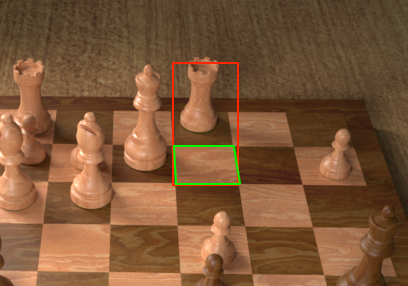
\includegraphics[width=\textwidth]{3828_annotated}
        \caption{region from the original image with marked square}
        \label{fig:occupancy_classification_fp_original}
    \end{subfigure}
    \hfill
    \begin{subfigure}[b]{0.3\textwidth}
        \centering
        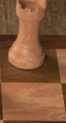
\includegraphics[width=.7\textwidth]{3828_cut}
        \caption{cropped sample}
        \label{fig:occupancy_classification_fp_cropped}
    \end{subfigure}
    \caption[An example illustrating why an immediate piece classification approach is prone to reporting false positives.]{An example illustraing why an immediate piece classification approach is prone to reporting false positives. Consider the square marked in green in the original image \subref{fig:occupancy_classification_fp_original}. The bounding box for piece classification (marked in red) must be quite tall because the square might contain a tall piece such as a queen or king (the box must be at least as tall as the queen in the adjacent square on the left). The resulting sample, depicted in \subref{fig:occupancy_classification_fp_cropped}, contains almost the entire rook of the square behind. Thus, a piece classifier might classify this square as containing a rook instead of being empty.}
    \label{fig:occupancy_classification_fp}
\end{figure}
One common scenario where the trained classifier failed is illustrated in \cref{fig:occupancy_classification_fp}.
Notice that squares further away from the camera must be cropped with increasingly taller bounding boxes.
If a particular square is empty but its bounding box includes the piece from the adjacent square as in \cref{fig:occupancy_classification_fp_cropped}, the trained classifier was prone to report a false positive.

To solve this problem, a binary classifier is trained on cropped squares to decide whether they are empty or not.
Before cutting out the squares from the original image, the input image is warped to a two-dimensional overhead view by means of the projective transformation outlined in \cref{sec:find_homography}.
This ensures that all squares are of equal size and that the corners form right angles (which is not the case in the original image due to perspective distortion), as depicted in \cref{fig:occupancy_classification_samples_original,fig:occupancy_classification_samples_warped}.

\begin{figure}
    \centering
    \begin{subfigure}[b]{0.47\textwidth}
        \centering
        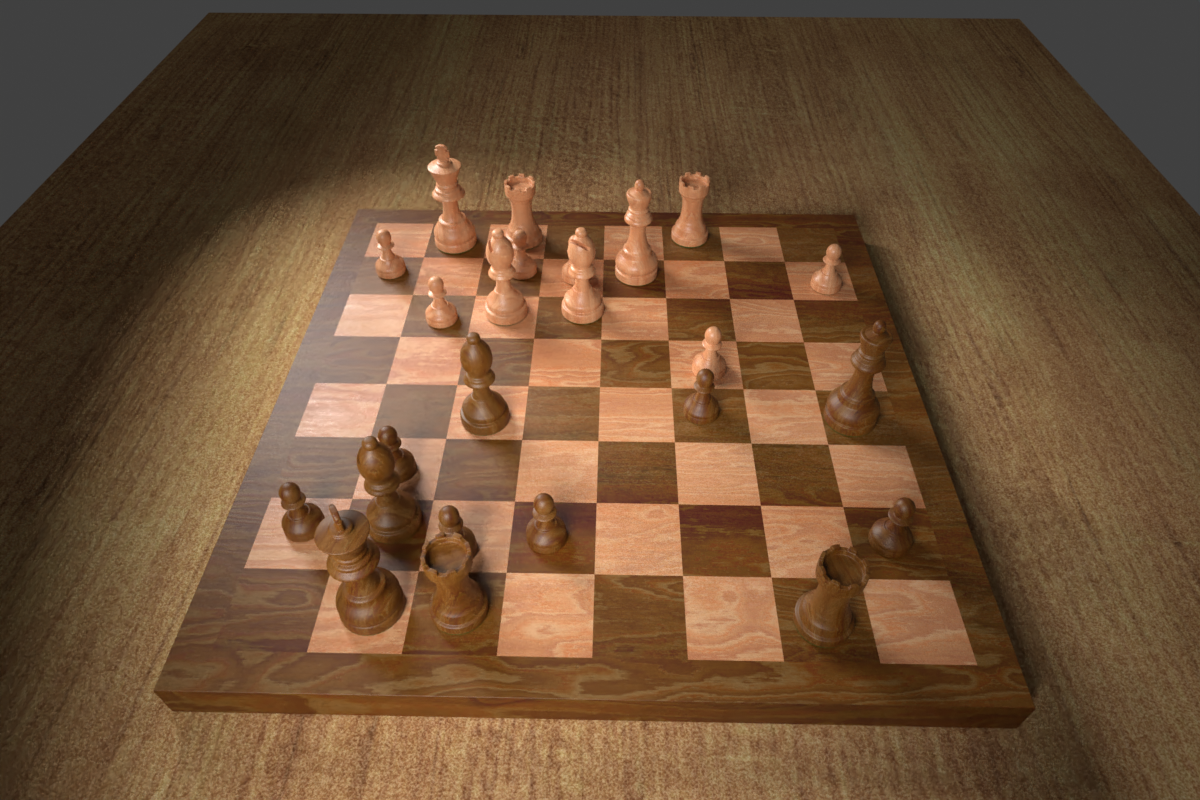
\includegraphics[width=\textwidth]{3828}
        \caption{original}
        \label{fig:occupancy_classification_samples_original}
    \end{subfigure}
    \hfill
    \begin{subfigure}[b]{0.47\textwidth}
        \centering
        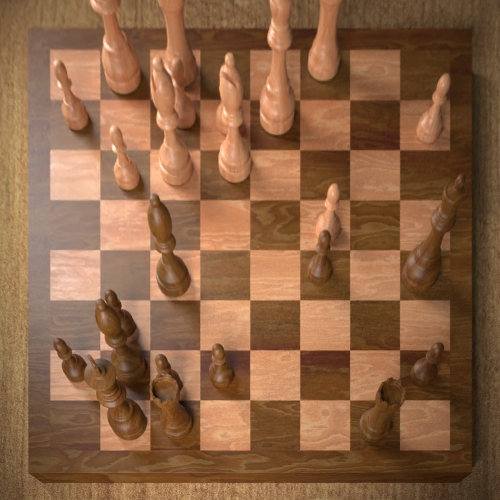
\includegraphics[width=\textwidth]{3828_unwarped}
        \caption{warped}
        \label{fig:occupancy_classification_samples_warped}
    \end{subfigure}
    
    \bigskip
    \begin{subfigure}[b]{0.47\textwidth}
        \centering
        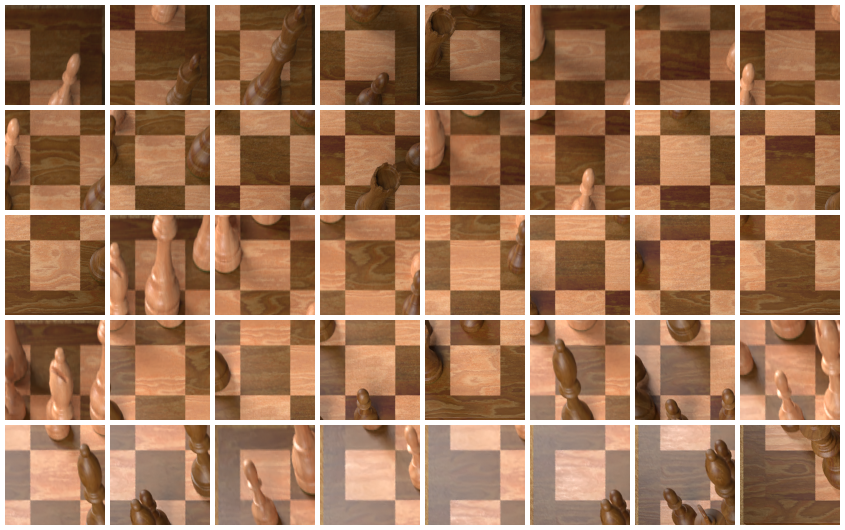
\includegraphics[width=\textwidth]{3828_empty}
        \caption{all 32 empty samples}
        \label{fig:occupancy_classification_samples_empty}
    \end{subfigure}
    \hfill
    \begin{subfigure}[b]{0.47\textwidth}
        \centering
        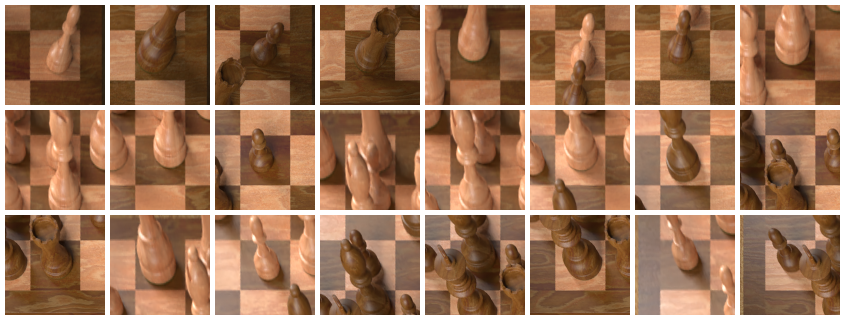
\includegraphics[width=\textwidth]{3828_occupied}
        \caption{all 24 occupied samples}
        \label{fig:occupancy_classification_samples_occupied}
    \end{subfigure}
    \caption[The process of obtaining samples for occupancy classification from a chessboard image.]{The process of obtaining samples for occupancy classification from a chessboard image. First, the original image \subref{fig:occupancy_classification_samples_original} is warped to a two-dimensional overhead view, \subref{fig:occupancy_classification_samples_warped}. Then, all squares are cropped (with a 50\% increase in width and height to include contextual information). Finally, the cropped squares are annoted using the \gls{fen} ground truth as either empty \subref{fig:occupancy_classification_samples_empty} or occupied \subref{fig:occupancy_classification_samples_occupied}.}
    \label{fig:occupancy_classification_samples}
\end{figure}

Cropping the squares from the warped image is trivial because the squares are of equal size.
In training the occupancy classifiers, we hypothesise that it would be useful to include contextual information with each square; therefore, the squares are not cropped tightly around their boundaries but instead with a 50\% increase in length on all four sides, as shown in \cref{fig:occupancy_classification_samples_empty,fig:occupancy_classification_samples_occupied}.
This might aid the classifier's decision in difficult situations where a chess piece from another square reaches into the cropped one due to the camera perspective.

\subsection{Designing and training \glspl{cnn}}
\label{sec:occupancy_cnns}
Six \gls{cnn} architectures are devised for the occupancy classification task, of which two accept $100\times 100$ pixel input images and the remaining four require the images to be of size $50\times 50$ pixels.
They differ in the number of convolution layers, pooling layers, and fully connected layers.
When referring to these models, we shall use a 4-tuple consisting of the input side length and the three aforementioned criteria.
\Cref{fig:occupancy_convnet} depicts the architecture of \acs{cnn} $(100, 3, 3, 3)$ which achieves the greatest validation accuracy of these six models.
\begin{figure}
    \centering
    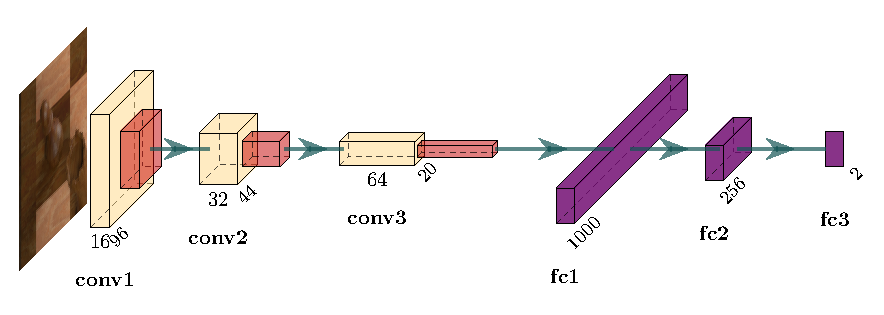
\includegraphics[width=\textwidth]{occupancy_convnet}
    \caption[Architecture of the CNN $(100,3,3,3)$ network for occupancy classification.]{
        Architecture of the \gls{cnn} $(100,3,3,3)$ network for occupancy classification.
        The input is a three-channel \gls{rgb} image with $100\times 100$ pixels.
        There are two convolutional layers (yellow) with a kernal size of $5 \times 5$ and stride $1$, meaning that each convolutional layer reduces the width and height by $4$.
        The final convolutional layer has a kernel size of $3 \times 3$, thus only reducing the input size by two.
        Starting with 16 filters in the first convolutional layer, the number of channels is doubled in each subsequent layer, as is common practice in \glspl{cnn} \cite{simonyan2015}.
        Each convolutional layer uses the \gls{relu} activation function and is followed by a max pooling layer with a $2\times 2$ kernel that is moved with a stride of $2$ such that the width and height are halved.
        Finally, the output of the last pooling layer is reshaped to a 640,000-dimensional vector that passes through two fully connected \gls{relu}-activated layers before reaching the final fully connected layer with softmax activation.
    }
    \label{fig:occupancy_convnet}
\end{figure}
The final fully connected layer in each model contains two output units that represent the two classes (occupied and empty).
The models are trained using the cross-entropy loss function on the outputs.
Training proceeds using the popular \emph{Adam} optimizer \cite{kingma2017} with a learning rate of $0.001$ for three whole passes over the training set using a batch size of 128.
At every 100 steps, the model's loss and accuracy is computed over the entire validation set, the results of which are reported in \cref{fig:occupancy_cnn_loss_accuracy}.
\begin{figure}
    \makebox[\textwidth][c]{
        \begin{subfigure}{.45\textwidth}
            \begin{tikzpicture}
                \begin{axis}[
                    no markers,
                    xlabel={step},
                    ylabel={cross-entropy loss},
                    title={Loss},
                    scale only axis,
                    width=.9\textwidth,
                    legend style={at={(0.98,0.98)},anchor=north east}
                ]
                    \addplot table [x=Step, y=Value, col sep=comma] {data/run-occupancy_classifier_CNN100_3Conv_3Pool_3FC_train-tag-Loss.csv};
                    \addplot table [x=Step, y=Value, col sep=comma] {data/run-occupancy_classifier_CNN100_3Conv_3Pool_3FC_val-tag-Loss.csv};
                    \legend{training,validation}
                \end{axis}
            \end{tikzpicture}
        \end{subfigure}
        \hfill
        \begin{subfigure}{.45\textwidth}
            \begin{tikzpicture}
                \begin{axis}[
                    no markers,
                    xlabel={step},
                    ylabel={accuracy},
                    title={Accuracy},
                    scale only axis,
                    width=.9\textwidth,
                    ylabel near ticks,
                    yticklabel pos=right,
                    legend style={at={(0.98,0.02)},anchor=south east}
                ]
                    \addplot table [x=Step, y=Value, col sep=comma] {data/run-occupancy_classifier_CNN100_3Conv_3Pool_3FC_train-tag-Accuracy.csv};
                    \addplot table [x=Step, y=Value, col sep=comma] {data/run-occupancy_classifier_CNN100_3Conv_3Pool_3FC_val-tag-Accuracy.csv};
                    \legend{training,validation}
                \end{axis}
            \end{tikzpicture}
        \end{subfigure}
    }
    \caption[Loss and accuracy during training on both the training and validation sets for the CNN $(100,3,3,3)$ model.]{Loss and accuracy during training on both the training and validation sets for the \gls{cnn} $(100,3,3,3)$ model. The best validation accuracy is 99.71\%.}
    \label{fig:occupancy_cnn_loss_accuracy}
\end{figure}
The model converges smoothly to a very low loss value, achieving a training accuracy of 99.70\% and validation accuracy of 99.71\%.
Due to the fact that the difference between training and validation accuracy is very small (in fact, the validation accuracy even happens to be slightly above the training accuracy), we conclude that the model does not overfit the training set.

\subsection{Transfer learning on deeper models}
\label{sec:occupancy_transfer_learning}
Apart from training custom \gls{cnn} architectures as described in the previous section, we examine whether fine-tuning pre-trained models on our dataset can achieve even better performances.
\Cref{sec:background_transfer_learning} explains the motivation for employing transfer learning and the general methodology of initialising the network with the pre-trained weights, then training just the classification head and finally training the whole network.
We replace the final layer of the pre-trained model's classification head with a fully-connected layer that has two output units so the network can classify `empty' and `occupied' squares.
Due to the abundance of data in the training set, it suffices to train the classification head for only one epoch (one pass over the dataset) with a learning rate $\alpha=10^{-3}$, followed by training the whole network for two epochs\footnote{The number of steps is significantly greater than the number of epochs because each epoch is split into multiple batches.} with $\alpha=10^{-4}$.
As underlying models, we compare the popular \gls{cnn} architectures
VGG \cite{simonyan2015},
ResNet \cite{he2016}, and
AlexNet \cite{krizhevsky2017}.
The weights in each case were pretrained on the ImageNet \cite{deng2009} dataset.

The ResNet model achieves the highest validation accuracy (99.96\%) of all evaluated architectures.
Training progresses smoothly and there is no significant gap between the training and validation metrics which are depicted in \cref{fig:occupancy_resnet_loss_accuracy}.
\begin{figure}
    \makebox[\textwidth][c]{
        \begin{subfigure}{.45\textwidth}
            \begin{tikzpicture}
                \begin{axis}[
                    no markers,
                    xlabel={step},
                    ylabel={cross-entropy loss},
                    title={Loss},
                    scale only axis,
                    width=.9\textwidth,
                    legend style={at={(0.98,0.98)},anchor=north east}
                ]
                    \addplot table [x=Step, y=Value, col sep=comma] {data/run-occupancy_classifier_ResNet_train-tag-Loss.csv};
                    \addplot table [x=Step, y=Value, col sep=comma] {data/run-occupancy_classifier_ResNet_val-tag-Loss.csv};
                    \legend{training,validation}
                \end{axis}
            \end{tikzpicture}
        \end{subfigure}
        \hfill
        \begin{subfigure}{.45\textwidth}
            \begin{tikzpicture}
                \begin{axis}[
                    no markers,
                    xlabel={step},
                    ylabel={accuracy},
                    title={Accuracy},
                    scale only axis,
                    width=.9\textwidth,
                    ylabel near ticks,
                    yticklabel pos=right,
                    legend style={at={(0.98,0.02)},anchor=south east}
                ]
                    \addplot table [x=Step, y=Value, col sep=comma] {data/run-occupancy_classifier_ResNet_train-tag-Accuracy.csv};
                    \addplot table [x=Step, y=Value, col sep=comma] {data/run-occupancy_classifier_ResNet_val-tag-Accuracy.csv};
                    \legend{training,validation}
                \end{axis}
            \end{tikzpicture}
        \end{subfigure}
    }
    \caption[Loss and accuracy during training on both the training and validation sets for the ResNet model.]{Loss and accuracy during training on both the training and validation sets for the ResNet model. The best validation accuracy is 99.96\%.}
    \label{fig:occupancy_resnet_loss_accuracy}
\end{figure}
The large decrease in loss and simultaneous increase in accuracy that occurs just after step 2,000 in that figure coincides with the transition from training exclusively the classification head to the whole network.
After that, the model converges smoothly to a low loss and high accuracy.
The final model misclassifies only four of the 146 samples in the validation set; these are shown in \cref{fig:occupancy_resnet_mistakes}.
\begin{figure}
    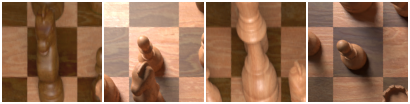
\includegraphics[width=\textwidth]{ResNet_val_mistakes.png}
    \caption[The four samples that the ResNet model misclassified in the validation set.]{The four samples that the ResNet model misclassified in the validation set of size 146. The left sample depicts an empty square, and the remaining three are of occupied squares.}
    \label{fig:occupancy_resnet_mistakes}
\end{figure}

\subsection{Analysis}
Each model is trained separately on the dataset of squares that are cropped to include contextual information (by increasing the bounding box by 50\% in each direction), and the same samples except that the squares are cropped tightly.
Key performance metrics for each model are summarised in \cref{tbl:occupancy_classifier_performance}.
\begin{table}
    \centering
    \makebox[\textwidth][c]{
        \pgfplotstabletypeset[
            col sep=tab,
            columns={context,model,parameters,val_accuracy,val_precision/occupied,val_recall/occupied,val_misclassified,train_accuracy},
            every head row/.style={%
                before row=\toprule,
                after row=\midrule%
            },
            every last row/.style={
                after row=\bottomrule
            },
            columns/model/.style={
                string type
            },
            columns/parameters/.style={
                column name={\makecell{\# trainable\\parameters}}
            },
            columns/context/.style={
                string type,
                column name={}
            },
            columns/val_accuracy/.style={
                dec sep align,
                postproc cell content/.append code={
                    \ifnum1=\pgfplotstablepartno
                        \pgfkeysalso{@cell content/.add={}{\%}}%
                    \fi
                },
                fixed,
                fixed zerofill,
                column name={accuracy}
            },
            columns/train_accuracy/.style={
                dec sep align,
                postproc cell content/.append code={
                    \ifnum1=\pgfplotstablepartno
                        \pgfkeysalso{@cell content/.add={}{\%}}%
                    \fi
                },
                fixed,
                fixed zerofill,
                column name={\makecell{training \\ accuracy}}
            },
            columns/val_precision/occupied/.style={
                dec sep align,
                precision=3,
                fixed,
                fixed zerofill,
                column name={precision}
            },
            columns/val_recall/occupied/.style={
                dec sep align,
                precision=3,
                fixed,
                fixed zerofill,
                column name={recall}
            },
            columns/val_misclassified/.style={
                column name={\makecell{errors}}
            },
        ]{data/occupancy_classifier.dat}
    }
    \caption[Performance of all occupancy classification models on the validation set.]{
        Performance of all occupancy classification models on the validation set.
        For the \gls{cnn} models, the 4-tuple denotes the length of the square input size in pixels, the number of convolution layers, the number of pooling layers, and the number of fully connected layers.
        The check mark in the left column indicates whether the input samples contained contextual information (cropped to include part of the adjacent squares).
        In the penultimate column, the total number of misclassifications in the validation set are reported (the validation set consists of 9,346 samples).
        The training accuracy is given in the rightmost column for comparison.
        Notice that there is no significant difference between the validation and training accuracies, indicating that none of the models suffer from overfitting.
    }
    \label{tbl:occupancy_classifier_performance}
\end{table}
In each case, the model trained on the samples that contained contexual information outperfomed its counterpart trained on tightly cropped samples, confirming the hypothesis voiced at the beginning of \cref{sec:occupancy_classification} that the information around the square itself is useful.

Furthermore, we see that the pre-trained models from \cref{sec:occupancy_transfer_learning} perform better than the \glspl{cnn} from \cref{sec:occupancy_cnns}, although the differences in accuracy are small and every model achieves accuracies above 99\%.
Likely reasons for the superiority of the pre-trained models are the increased number of trainable parameters (up to two orders of magnitude higher than the simple \glspl{cnn}), the use of transfer learning, and the more complex architectural designs.
Nonetheless, we see in \cref{tbl:occupancy_classifier_performance} by comparing the training and validation accuracies that none of the models suffer from overfitting which is not suprising given the size of the dataset.
We select the ResNet model for use in the chess recognition pipeline because it attains the highest accuracy score.


\section{Piece classification}
\label{sec:piece_classification}
Now that the occupancy of each square on the chessboard can be detected to a high degree of accuracy, the next step is to classify the piece in each of the occupied squares.
We require a 12-way classifier that takes as input a cropped image of an occupied square and outputs the chess piece on that square. 
There are six types of chess pieces (pawn, knight, bishop, rook, queen, and king), and each piece can either be white or black in colour, thus there are a dozen classes.

We must pay some special attention to how the pieces are cropped. 
Simply following the approach described in \cref{sec:occupancy_classification} would provide insufficient information to classify pieces.
Especially tall pieces at the back of the board would be cropped in a manner such that only the bottom part of the piece remains in the \gls{roi}. 
Consider for example the white king in \cref{fig:occupancy_classification_samples}.
Cropping only the square it is located in would not include its crown which is an important feature needed to distinguish between kings and queens.
Instead, we must choose a rectangular bounding box that is tall enough to account for the perspective distortion.

The camera perspective causes another phenomenon that we must account for: pieces on the left of the board tend to `slant' to the left, and vice-versa on the right.
This is due to the vanishing point of the normal vectors on the chessboard surface being roughly centred horizontally with regards to the location of the chessboard itself%
\footnote{%
    Unfortunately, it is not possible to compute the vanishing point of the normals based solely on the information available in the input images as this would require knowledge of the intrinsic and extrinsic camera parameters \cite{hartley2004}.
    The aim of this work is to recognise chess positions from just the input image without any further information; therefore, we devise a heuristic based on the observation that the vanishing point tends to be vertically below the chessboard and roughly horizontally centred.
}, as illustrated in \cref{fig:occupancy_classification_normals}.
\begin{figure}
    \centering
    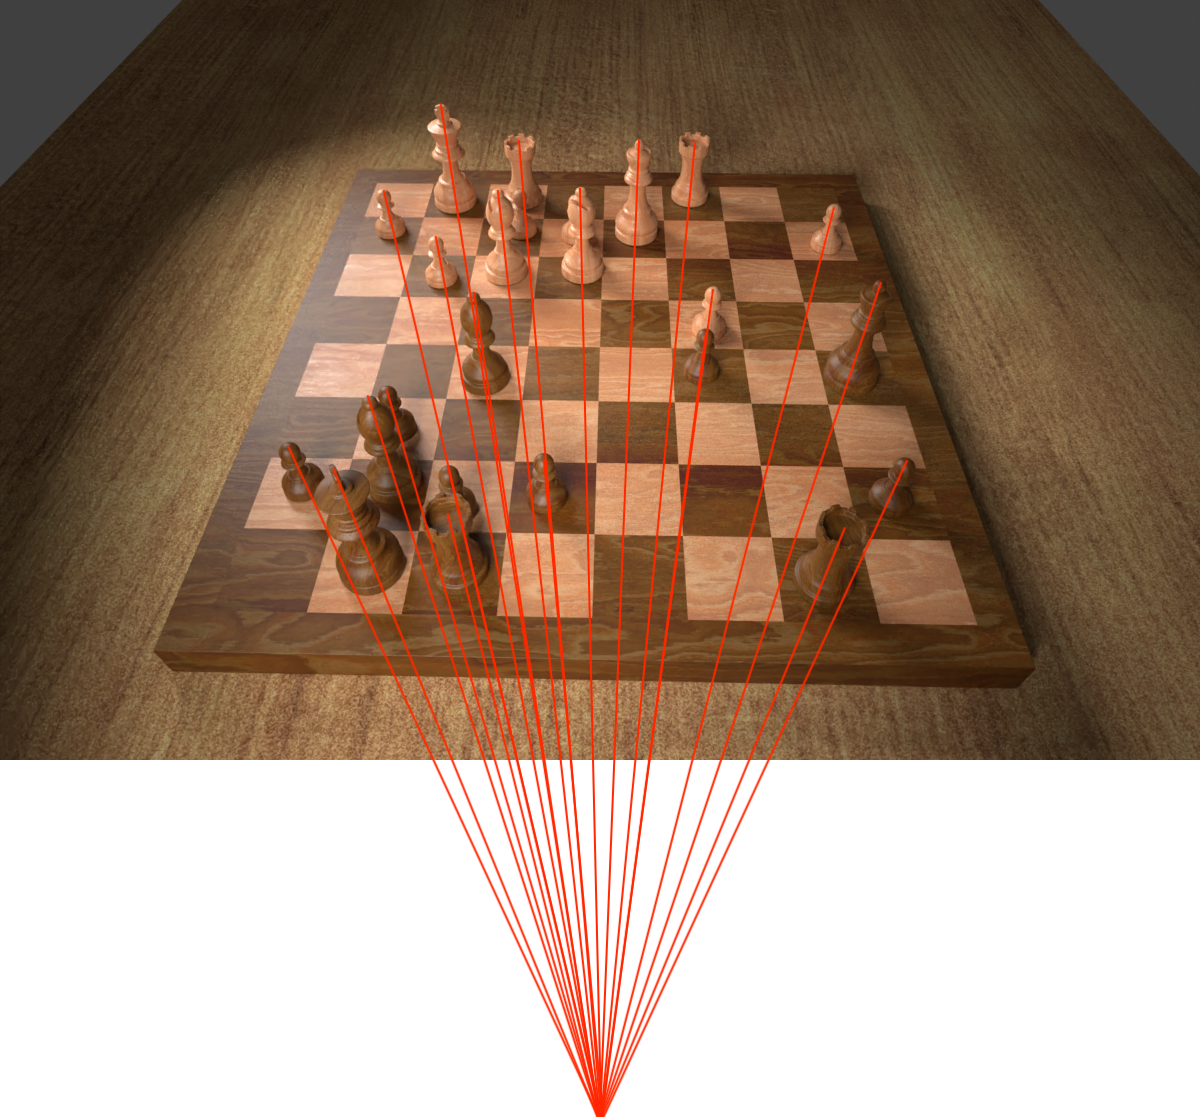
\includegraphics[width=.7\textwidth]{3828_normals.png}
    \caption[The normals of the chessboard surface converge to a single vanishing point which is below the image.]{The normals of the chessboard surface (corresponding to the direction the pieces are pointing, marked in red) converge to a single vanishing point which is below the image. We assume that the vanishing point is roughly horizontally centred with the chessboard, as this corresponds to how chessboards are usually photographed. As a result, pieces on left `lean' left, and vice-versa on the right.}
    \label{fig:occupancy_classification_normals}
\end{figure}
Hence, we must extend the \gls{roi} horizontally in the appropriate direction.

To obtain the \glspl{roi}, we first warp the input image of the chessboard as described in \cref{sec:occupancy_classification} and exemplified in \cref{fig:occupancy_classification_samples_warped}.
At first, each piece's bounding box corresponds to the square it is located on, i.e.\ its width and height are that of the square\footnote{Note that due to the warped perspective, all squares have equal width and height.}.
Depending on the rank $r$, the height is increased by
\begin{equation*}
    h_\text{inc}(r) = \frac{2r + 5}{7}
\end{equation*}
where the unit of measurement corresponds to the warped coordinate system described in \cref{sec:homography_matrix} (each chess square is one square unit).
This represents an arithmetic progression such that the bounding box for pieces in the first rank (bottom row of the chessboard, i.e.\ $r=1$) is increased by one square, and pieces in the top row ($r=8$) have their height increased by three units.

The increase in width is dependent on the file $f$ and given by the piecewise-defined arithmetic progression
\begin{equation*}
    w_\text{inc}(f) = \begin{cases}
        -\frac{f}{4} & f \leq 4 \\
        \frac{f-4}{4} & f > 4.
    \end{cases}
\end{equation*}
A negative increase in width means that the bounding box is extended to the left, whereas a positive increase means it is widened to the right.
Thus, pieces on the left half of the board ($1 \leq f \leq 4$) have their bounding boxes extended to the left, and vice-versa on the right (for $4 < f \leq 8$).

Experiments demonstrate that this heuristic generates bounding boxes that are large enough to contain even the tallest pieces in most cases, whilst not being needlessly large.
As a further preprocessing step, the cropped \glspl{roi} for all pieces on the left side of the board ($1 \leq f \leq 4$) are flipped vertically, such that the square that the piece stands on is always in the bottom left of the image.
This may help the classifier understand what piece is being referred to in samples where the larger bounding box includes adjacent pieces in the image.
\Cref{fig:white_queens} shows a random selection of the \glspl{roi} corresponding to white queens in order to demonstrate that the bounding boxes are large enough to contain even tall pieces.
\begin{figure}
    \centering
    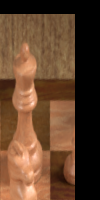
\includegraphics[width=.15\textwidth]{white_queen_1.png}
    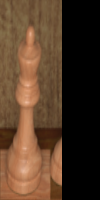
\includegraphics[width=.15\textwidth]{white_queen_2.png}
    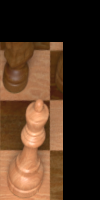
\includegraphics[width=.15\textwidth]{white_queen_3.png}
    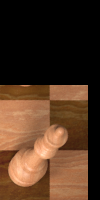
\includegraphics[width=.15\textwidth]{white_queen_4.png}
    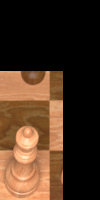
\includegraphics[width=.15\textwidth]{white_queen_5.png}
    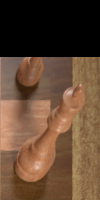
\includegraphics[width=.15\textwidth]{white_queen_6.png}
    \caption[A random selection of six samples of white queens in the training set.]{A random selection of six samples of white queens in the training set. Notice that the square each queen is located on is always in the bottom left of the image and of uniform dimensions across all samples.}
    \label{fig:white_queens}
\end{figure}

\subsection{\glsentryshort{cnn} models}
Similar to \cref{sec:occupancy_classification}, we train several \glspl{cnn} for the piece classification task.
However, since the problem is not binary anymore, the final layer of our \glspl{cnn} must have 12 instead of two output units.
For the pre-trained models, we follow the same two-stage training regime, but double the number of epochs at each stage, so that the classification head is trained for two epochs followed by the whole network for four epochs.
Furthermore, we introduce one more architecture, InceptionV3 \cite{szegedy2016}, that is a bit more complicated to train due to its use of batch normalisation and multiple losses.
The exact details are, however, beyond the scope of this report.
All other configurations are as described in \cref{sec:occupancy_classification}.

In total, we train six models, two of which are `vanilla' \glspl{cnn} (the best two from \cref{sec:occupancy_classification} are selected for this task), and the rest are deeper models trained by means of transfer learning.
The results in \cref{tbl:piece_classifier_performance} indicate a more significant difference between the hand-crafted \glspl{cnn} and the deeper models (around three percentage points) than was the case for the occupancy classifier.
\begin{table}
    \centering
    \makebox[\textwidth][c]{
        \pgfplotstabletypeset[
            col sep=tab,
            columns={model,parameters,val_accuracy,val_misclassified,train_accuracy},
            every head row/.style={%
                before row=\toprule,
                after row=\midrule%
            },
            every last row/.style={
                after row=\bottomrule
            },
            columns/model/.style={
                string type
            },
            columns/parameters/.style={
                column name={\makecell{\# trainable\\parameters}}
            },
            columns/val_accuracy/.style={
                dec sep align,
                postproc cell content/.append code={
                    \ifnum1=\pgfplotstablepartno
                        \pgfkeysalso{@cell content/.add={}{\%}}%
                    \fi
                },
                fixed,
                fixed zerofill,
                column name={accuracy}
            },
            columns/train_accuracy/.style={
                dec sep align,
                postproc cell content/.append code={
                    \ifnum1=\pgfplotstablepartno
                        \pgfkeysalso{@cell content/.add={}{\%}}%
                    \fi
                },
                fixed,
                fixed zerofill,
                column name={\makecell{training \\ accuracy}}
            },
            columns/val_misclassified/.style={
                column name={\makecell{errors}}
            },
        ]{data/piece_classifier.dat}
    }
    \caption[Performance of all piece classifiers on the validation set.]{
        Performance of all piece classifiers on the validation set.
    }
    \label{tbl:piece_classifier_performance}
\end{table}
The InceptionV3 model achieves the best performance with a validation accuracy of 100\%, i.e.\ there were no misclassifications in the validation set.
Therefore, we adopt that model in the chess recognition pipeline.
\Cref{fig:pieces_inception_loss_accuracy} shows the development of loss and accuracy during training. 
\begin{figure}
    \makebox[\textwidth][c]{
        \begin{subfigure}{.45\textwidth}
            \begin{tikzpicture}
                \begin{axis}[
                    no markers,
                    xlabel={step},
                    ylabel={cross-entropy loss},
                    title={Loss},
                    scale only axis,
                    width=.9\textwidth,
                    legend style={at={(0.98,0.98)},anchor=north east}
                ]
                    \addplot table [x=Step, y=Value, col sep=comma] {data/run-piece_classifier_InceptionV3_train-tag-Loss.csv};
                    \addplot table [x=Step, y=Value, col sep=comma] {data/run-piece_classifier_InceptionV3_val-tag-Loss.csv};
                    \legend{training,validation}
                \end{axis}
            \end{tikzpicture}
        \end{subfigure}
        \hfill
        \begin{subfigure}{.45\textwidth}
            \begin{tikzpicture}
                \begin{axis}[
                    no markers,
                    xlabel={step},
                    ylabel={accuracy},
                    title={Accuracy},
                    scale only axis,
                    width=.9\textwidth,
                    ylabel near ticks,
                    yticklabel pos=right,
                    legend style={at={(0.98,0.02)},anchor=south east}
                ]
                    \addplot table [x=Step, y=Value, col sep=comma] {data/run-piece_classifier_InceptionV3_train-tag-Accuracy.csv};
                    \addplot table [x=Step, y=Value, col sep=comma] {data/run-piece_classifier_InceptionV3_val-tag-Accuracy.csv};
                    \legend{training,validation}
                \end{axis}
            \end{tikzpicture}
        \end{subfigure}
    }
    \caption[Loss and accuracy during training on both the training and validation sets for the InceptionV3 model.]{Loss and accuracy during training on both the training and validation sets for the InceptionV3 model. The best validation accuracy is 100.00\%.}
    \label{fig:pieces_inception_loss_accuracy}
\end{figure}
Similar to the ResNet occupancy classifier in \cref{fig:occupancy_resnet_loss_accuracy}, we witness an abrupt drop in loss and simultaneous increase in accuracy when all remaining layers are unfrozen.
This occurs earlier in the training of the piece classifier because the size of the dataset is smaller\footnote{The dataset for piece classification consists of only occupied squares whereas the occupancy classification dataset comprises all squares.}.
\Cref{fig:pieces_inception_loss_accuracy} also exhibits a higher degree of small fluctuations around the loss and accuracy curves which can be attributed to the increased difficulty of this task where we must classify a dozen different piece types.

\section{Producing a prediction}
\label{sec:preparing_results}
\Cref{sec:board_localisation,sec:occupancy_classification,sec:piece_classification} describe the three components of the chess recognition pipeline.
Assembling these parts facilitates an end-to-end chess recognition system that takes an input image and ultimately produces a \gls{fen} prediction.
First, we localise the board (\cref{sec:board_localisation}) and obtain the pixel coordinates of the four chessboard corners.
Then, we warp the input image to fit the chessboard on a regular grid.
We crop each of the squares and feed them to the occupancy classifier (\cref{sec:occupancy_classification}).
The output is a probability for the occupancy of each square.
We retain only the squares with an occupancy probability over 50\% and cut out the corresponding squares in the same manner as the piece classification dataset was created in \cref{sec:piece_classification}.
After that, each of the occupied samples is supplied to the piece classifier in order to obtain a probability distribution over the piece types.
In each instance, we simply use the class with the highest probability.
Finally, we create an internal representation of the chessboard based on the results of the two classifiers in order to produce a \gls{fen} description of the position on the board.

\Cref{tbl:chess_recognition_trainval_results} summarises key performance metrics of the end-to-end chess recognition pipeline evaluated on both the training and validation sets (the test set is evaluated in \cref{chap:evaluation}).
\begin{table}
    \makebox[\textwidth][c]{
        \begin{tabular}{lrr}
            \toprule
            metric & training set & validation set \\
            \midrule
            mean number of incorrect squares per board           & 0.27    & 0.03 \\
            percentage of boards predicted with no mistakes      & 94.77\% & 97.95\%   \\
            percentage of boards predicted with $\leq 1$ mistake & 99.14\% & 99.32\%   \\
            per-board corner detection accuracy                  & 99.59\% & 100.00\% \\
            per-square occupancy classification accuracy         & 99.81\% & 99.97\% \\
            per-square piece classification accuracy             & 99.99\% & 99.99\% \\
            \bottomrule
        \end{tabular}
    }
    \caption[Performance of the chess recognition pipeline on the training and validation sets.]{Performance of the chess recognition pipeline on the training and validation sets. The accuracies of the piece and occupancy classifiers are reported on a per-square basis, and in computing the accuracy of the piece classifier, we consider only the squares that were marked as `occupied' by the occupancy classifier. This is because the piece classifier is used only on the occupied squares.}
    \label{tbl:chess_recognition_trainval_results}
\end{table}
On average, the pipeline misclassifies only 0.03 squares per board.
Overall, 98\% of the chessboards in the validation set are predicted without mistakes, and 2\% of the samples had only one incorrect square.
The accuracies of the two classifiers as well as the corner dectector is above 99\%.

\end{document}